% REV00 Tue 04 May 2021 13:55:16 WIB
% START Tue 04 May 2021 13:55:16 WIB

\chapter{XXX}

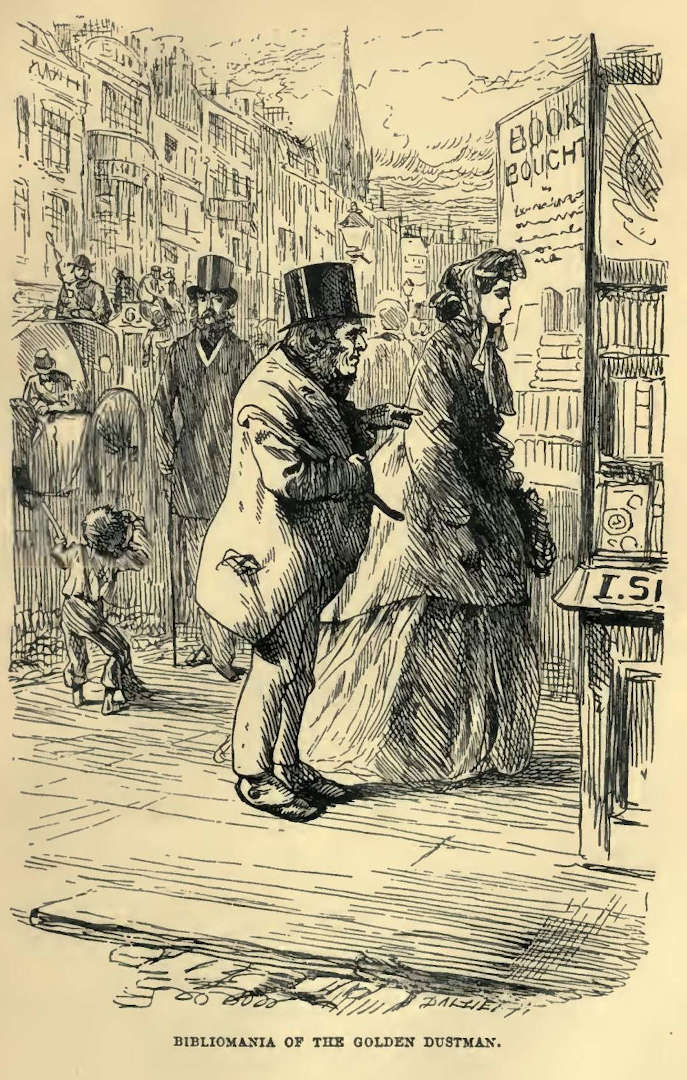
\includegraphics[scale=2.3]{03-05-01}

Chapter 17

A SOCIAL CHORUS


Amazement sits enthroned upon the countenances of Mr and Mrs Alfred
Lammle’s circle of acquaintance, when the disposal of their first-class
furniture and effects (including a Billiard Table in capital letters),
‘by auction, under a bill of sale,’ is publicly announced on a waving
hearthrug in Sackville Street. But, nobody is half so much amazed as
Hamilton Veneering, Esquire, M.P. for Pocket-Breaches, who instantly
begins to find out that the Lammles are the only people ever entered on
his soul’s register, who are NOT the oldest and dearest friends he has
in the world. Mrs Veneering, W.M.P. for Pocket-Breaches, like a faithful
wife shares her husband’s discovery and inexpressible astonishment.
Perhaps the Veneerings twain may deem the last unutterable feeling
particularly due to their reputation, by reason that once upon a time
some of the longer heads in the City are whispered to have shaken
themselves, when Veneering’s extensive dealings and great wealth were
mentioned. But, it is certain that neither Mr nor Mrs Veneering can
find words to wonder in, and it becomes necessary that they give to the
oldest and dearest friends they have in the world, a wondering dinner.

For, it is by this time noticeable that, whatever befals, the Veneerings
must give a dinner upon it. Lady Tippins lives in a chronic state
of invitation to dine with the Veneerings, and in a chronic state of
inflammation arising from the dinners. Boots and Brewer go about in
cabs, with no other intelligible business on earth than to beat up
people to come and dine with the Veneerings. Veneering pervades the
legislative lobbies, intent upon entrapping his fellow-legislators to
dinner. Mrs Veneering dined with five-and-twenty bran-new faces over
night; calls upon them all to day; sends them every one a dinner-card
to-morrow, for the week after next; before that dinner is digested,
calls upon their brothers and sisters, their sons and daughters, their
nephews and nieces, their aunts and uncles and cousins, and invites
them all to dinner. And still, as at first, howsoever, the dining circle
widens, it is to be observed that all the diners are consistent in
appearing to go to the Veneerings, not to dine with Mr and Mrs Veneering
(which would seem to be the last thing in their minds), but to dine with
one another.

Perhaps, after all,--who knows?--Veneering may find this dining, though
expensive, remunerative, in the sense that it makes champions.
Mr Podsnap, as a representative man, is not alone in caring very
particularly for his own dignity, if not for that of his acquaintances,
and therefore in angrily supporting the acquaintances who have taken out
his Permit, lest, in their being lessened, he should be. The gold and
silver camels, and the ice-pails, and the rest of the Veneering table
decorations, make a brilliant show, and when I, Podsnap, casually remark
elsewhere that I dined last Monday with a gorgeous caravan of camels,
I find it personally offensive to have it hinted to me that they are
broken-kneed camels, or camels labouring under suspicion of any sort. ‘I
don’t display camels myself, I am above them: I am a more solid man; but
these camels have basked in the light of my countenance, and how dare
you, sir, insinuate to me that I have irradiated any but unimpeachable
camels?’

The camels are polishing up in the Analytical’s pantry for the dinner
of wonderment on the occasion of the Lammles going to pieces, and Mr
Twemlow feels a little queer on the sofa at his lodgings over the stable
yard in Duke Street, Saint James’s, in consequence of having taken
two advertised pills at about mid-day, on the faith of the printed
representation accompanying the box (price one and a penny halfpenny,
government stamp included), that the same ‘will be found highly salutary
as a precautionary measure in connection with the pleasures of the
table.’ To whom, while sickly with the fancy of an insoluble pill
sticking in his gullet, and also with the sensation of a deposit of warm
gum languidly wandering within him a little lower down, a servant enters
with the announcement that a lady wishes to speak with him.

‘A lady!’ says Twemlow, pluming his ruffled feathers. ‘Ask the favour of
the lady’s name.’

The lady’s name is Lammle. The lady will not detain Mr Twemlow longer
than a very few minutes. The lady is sure that Mr Twemlow will do her
the kindness to see her, on being told that she particularly desires
a short interview. The lady has no doubt whatever of Mr Twemlow’s
compliance when he hears her name. Has begged the servant to be
particular not to mistake her name. Would have sent in a card, but has
none.

‘Show the lady in.’ Lady shown in, comes in.

Mr Twemlow’s little rooms are modestly furnished, in an old-fashioned
manner (rather like the housekeeper’s room at Snigsworthy Park), and
would be bare of mere ornament, were it not for a full-length engraving
of the sublime Snigsworth over the chimneypiece, snorting at a
Corinthian column, with an enormous roll of paper at his feet, and a
heavy curtain going to tumble down on his head; those accessories being
understood to represent the noble lord as somehow in the act of saving
his country.

‘Pray take a seat, Mrs Lammle.’ Mrs Lammle takes a seat and opens the
conversation.

‘I have no doubt, Mr Twemlow, that you have heard of a reverse of
fortune having befallen us. Of course you have heard of it, for no kind
of news travels so fast--among one’s friends especially.’

Mindful of the wondering dinner, Twemlow, with a little twinge, admits
the imputation.

‘Probably it will not,’ says Mrs Lammle, with a certain hardened manner
upon her, that makes Twemlow shrink, ‘have surprised you so much as some
others, after what passed between us at the house which is now turned
out at windows. I have taken the liberty of calling upon you, Mr
Twemlow, to add a sort of postscript to what I said that day.’

Mr Twemlow’s dry and hollow cheeks become more dry and hollow at the
prospect of some new complication.

‘Really,’ says the uneasy little gentleman, ‘really, Mrs Lammle, I
should take it as a favour if you could excuse me from any further
confidence. It has ever been one of the objects of my life--which,
unfortunately, has not had many objects--to be inoffensive, and to keep
out of cabals and interferences.’

Mrs Lammle, by far the more observant of the two, scarcely finds it
necessary to look at Twemlow while he speaks, so easily does she read
him.

‘My postscript--to retain the term I have used’--says Mrs Lammle, fixing
her eyes on his face, to enforce what she says herself--‘coincides
exactly with what you say, Mr Twemlow. So far from troubling you with
any new confidence, I merely wish to remind you what the old one was. So
far from asking you for interference, I merely wish to claim your strict
neutrality.’

Twemlow going on to reply, she rests her eyes again, knowing her ears to
be quite enough for the contents of so weak a vessel.

‘I can, I suppose,’ says Twemlow, nervously, ‘offer no reasonable
objection to hearing anything that you do me the honour to wish to say
to me under those heads. But if I may, with all possible delicacy and
politeness, entreat you not to range beyond them, I--I beg to do so.’

‘Sir,’ says Mrs Lammle, raising her eyes to his face again, and quite
daunting him with her hardened manner, ‘I imparted to you a certain
piece of knowledge, to be imparted again, as you thought best, to a
certain person.’

‘Which I did,’ says Twemlow.

‘And for doing which, I thank you; though, indeed, I scarcely know why
I turned traitress to my husband in the matter, for the girl is a poor
little fool. I was a poor little fool once myself; I can find no better
reason.’ Seeing the effect she produces on him by her indifferent laugh
and cold look, she keeps her eyes upon him as she proceeds. ‘Mr Twemlow,
if you should chance to see my husband, or to see me, or to see both of
us, in the favour or confidence of any one else--whether of our common
acquaintance or not, is of no consequence--you have no right to use
against us the knowledge I intrusted you with, for one special purpose
which has been accomplished. This is what I came to say. It is not a
stipulation; to a gentleman it is simply a reminder.’

Twemlow sits murmuring to himself with his hand to his forehead.

‘It is so plain a case,’ Mrs Lammle goes on, ‘as between me (from the
first relying on your honour) and you, that I will not waste another
word upon it.’ She looks steadily at Mr Twemlow, until, with a shrug,
he makes her a little one-sided bow, as though saying ‘Yes, I think you
have a right to rely upon me,’ and then she moistens her lips, and shows
a sense of relief.

‘I trust I have kept the promise I made through your servant, that I
would detain you a very few minutes. I need trouble you no longer, Mr
Twemlow.’

‘Stay!’ says Twemlow, rising as she rises. ‘Pardon me a moment. I should
never have sought you out, madam, to say what I am going to say, but
since you have sought me out and are here, I will throw it off my mind.
Was it quite consistent, in candour, with our taking that resolution
against Mr Fledgeby, that you should afterwards address Mr Fledgeby as
your dear and confidential friend, and entreat a favour of Mr Fledgeby?
Always supposing that you did; I assert no knowledge of my own on the
subject; it has been represented to me that you did.’

‘Then he told you?’ retorts Mrs Lammle, who again has saved her eyes
while listening, and uses them with strong effect while speaking.

‘Yes.’

‘It is strange that he should have told you the truth,’ says Mrs
Lammle, seriously pondering. ‘Pray where did a circumstance so very
extraordinary happen?’

Twemlow hesitates. He is shorter than the lady as well as weaker, and,
as she stands above him with her hardened manner and her well-used eyes,
he finds himself at such a disadvantage that he would like to be of the
opposite sex.

‘May I ask where it happened, Mr Twemlow? In strict confidence?’

‘I must confess,’ says the mild little gentleman, coming to his answer
by degrees, ‘that I felt some compunctions when Mr Fledgeby mentioned
it. I must admit that I could not regard myself in an agreeable light.
More particularly, as Mr Fledgeby did, with great civility, which I
could not feel that I deserved from him, render me the same service that
you had entreated him to render you.’

It is a part of the true nobility of the poor gentleman’s soul to say
this last sentence. ‘Otherwise,’ he has reflected, ‘I shall assume the
superior position of having no difficulties of my own, while I know of
hers. Which would be mean, very mean.’

‘Was Mr Fledgeby’s advocacy as effectual in your case as in ours?’ Mrs
Lammle demands.

‘As ineffectual.’

‘Can you make up your mind to tell me where you saw Mr Fledgeby, Mr
Twemlow?’

‘I beg your pardon. I fully intended to have done so. The reservation
was not intentional. I encountered Mr Fledgeby, quite by accident, on
the spot.--By the expression, on the spot, I mean at Mr Riah’s in Saint
Mary Axe.’

‘Have you the misfortune to be in Mr Riah’s hands then?’

‘Unfortunately, madam,’ returns Twemlow, ‘the one money obligation to
which I stand committed, the one debt of my life (but it is a just debt;
pray observe that I don’t dispute it), has fallen into Mr Riah’s hands.’

‘Mr Twemlow,’ says Mrs Lammle, fixing his eyes with hers: which he would
prevent her doing if he could, but he can’t; ‘it has fallen into Mr
Fledgeby’s hands. Mr Riah is his mask. It has fallen into Mr Fledgeby’s
hands. Let me tell you that, for your guidance. The information may be
of use to you, if only to prevent your credulity, in judging another
man’s truthfulness by your own, from being imposed upon.’

‘Impossible!’ cries Twemlow, standing aghast. ‘How do you know it?’

‘I scarcely know how I know it. The whole train of circumstances seemed
to take fire at once, and show it to me.’

‘Oh! Then you have no proof.’

‘It is very strange,’ says Mrs Lammle, coldly and boldly, and with some
disdain, ‘how like men are to one another in some things, though their
characters are as different as can be! No two men can have less affinity
between them, one would say, than Mr Twemlow and my husband. Yet my
husband replies to me “You have no proof,” and Mr Twemlow replies to me
with the very same words!’

‘But why, madam?’ Twemlow ventures gently to argue. ‘Consider why
the very same words? Because they state the fact. Because you HAVE no
proof.’

‘Men are very wise in their way,’ quoth Mrs Lammle, glancing haughtily
at the Snigsworth portrait, and shaking out her dress before departing;
‘but they have wisdom to learn. My husband, who is not over-confiding,
ingenuous, or inexperienced, sees this plain thing no more than Mr
Twemlow does--because there is no proof! Yet I believe five women out of
six, in my place, would see it as clearly as I do. However, I will never
rest (if only in remembrance of Mr Fledgeby’s having kissed my hand)
until my husband does see it. And you will do well for yourself to see
it from this time forth, Mr Twemlow, though I CAN give you no proof.’

As she moves towards the door, Mr Twemlow, attending on her, expresses
his soothing hope that the condition of Mr Lammle’s affairs is not
irretrievable.

‘I don’t know,’ Mrs Lammle answers, stopping, and sketching out the
pattern of the paper on the wall with the point of her parasol; ‘it
depends. There may be an opening for him dawning now, or there may be
none. We shall soon find out. If none, we are bankrupt here, and must go
abroad, I suppose.’

Mr Twemlow, in his good-natured desire to make the best of it, remarks
that there are pleasant lives abroad.

‘Yes,’ returns Mrs Lammle, still sketching on the wall; ‘but I doubt
whether billiard-playing, card-playing, and so forth, for the means to
live under suspicion at a dirty table-d’hote, is one of them.’

It is much for Mr Lammle, Twemlow politely intimates (though greatly
shocked), to have one always beside him who is attached to him in all
his fortunes, and whose restraining influence will prevent him from
courses that would be discreditable and ruinous. As he says it, Mrs
Lammle leaves off sketching, and looks at him.

‘Restraining influence, Mr Twemlow? We must eat and drink, and dress,
and have a roof over our heads. Always beside him and attached in all
his fortunes? Not much to boast of in that; what can a woman at my age
do? My husband and I deceived one another when we married; we must bear
the consequences of the deception--that is to say, bear one another, and
bear the burden of scheming together for to-day’s dinner and to-morrow’s
breakfast--till death divorces us.’

With those words, she walks out into Duke Street, Saint James’s. Mr
Twemlow returning to his sofa, lays down his aching head on its slippery
little horsehair bolster, with a strong internal conviction that a
painful interview is not the kind of thing to be taken after the dinner
pills which are so highly salutary in connexion with the pleasures of
the table.

But, six o’clock in the evening finds the worthy little gentleman
getting better, and also getting himself into his obsolete little silk
stockings and pumps, for the wondering dinner at the Veneerings. And
seven o’clock in the evening finds him trotting out into Duke Street, to
trot to the corner and save a sixpence in coach-hire.

Tippins the divine has dined herself into such a condition by this time,
that a morbid mind might desire her, for a blessed change, to sup
at last, and turn into bed. Such a mind has Mr Eugene Wrayburn, whom
Twemlow finds contemplating Tippins with the moodiest of visages,
while that playful creature rallies him on being so long overdue at the
woolsack. Skittish is Tippins with Mortimer Lightwood too, and has raps
to give him with her fan for having been best man at the nuptials of
these deceiving what’s-their-names who have gone to pieces. Though,
indeed, the fan is generally lively, and taps away at the men in
all directions, with something of a grisly sound suggestive of the
clattering of Lady Tippins’s bones.

A new race of intimate friends has sprung up at Veneering’s since he
went into Parliament for the public good, to whom Mrs Veneering is very
attentive. These friends, like astronomical distances, are only to be
spoken of in the very largest figures. Boots says that one of them is a
Contractor who (it has been calculated) gives employment, directly and
indirectly, to five hundred thousand men. Brewer says that another of
them is a Chairman, in such request at so many Boards, so far apart,
that he never travels less by railway than three thousand miles a week.
Buffer says that another of them hadn’t a sixpence eighteen months ago,
and, through the brilliancy of his genius in getting those shares issued
at eighty-five, and buying them all up with no money and selling them
at par for cash, has now three hundred and seventy-five thousand
pounds--Buffer particularly insisting on the odd seventy-five, and
declining to take a farthing less. With Buffer, Boots, and Brewer, Lady
Tippins is eminently facetious on the subject of these Fathers of the
Scrip-Church: surveying them through her eyeglass, and inquiring whether
Boots and Brewer and Buffer think they will make her fortune if she
makes love to them? with other pleasantries of that nature. Veneering,
in his different way, is much occupied with the Fathers too, piously
retiring with them into the conservatory, from which retreat the word
‘Committee’ is occasionally heard, and where the Fathers instruct
Veneering how he must leave the valley of the piano on his left,
take the level of the mantelpiece, cross by an open cutting at the
candelabra, seize the carrying-traffic at the console, and cut up the
opposition root and branch at the window curtains.

Mr and Mrs Podsnap are of the company, and the Fathers descry in Mrs
Podsnap a fine woman. She is consigned to a Father--Boots’s Father,
who employs five hundred thousand men--and is brought to anchor on
Veneering’s left; thus affording opportunity to the sportive Tippins on
his right (he, as usual, being mere vacant space), to entreat to be told
something about those loves of Navvies, and whether they really do live
on raw beefsteaks, and drink porter out of their barrows. But, in spite
of such little skirmishes it is felt that this was to be a wondering
dinner, and that the wondering must not be neglected. Accordingly,
Brewer, as the man who has the greatest reputation to sustain, becomes
the interpreter of the general instinct.

‘I took,’ says Brewer in a favourable pause, ‘a cab this morning, and I
rattled off to that Sale.’

Boots (devoured by envy) says, ‘So did I.’

Buffer says, ‘So did I’; but can find nobody to care whether he did or
not.

‘And what was it like?’ inquires Veneering.

‘I assure you,’ replies Brewer, looking about for anybody else to
address his answer to, and giving the preference to Lightwood; ‘I assure
you, the things were going for a song. Handsome things enough, but
fetching nothing.’

‘So I heard this afternoon,’ says Lightwood.

Brewer begs to know now, would it be fair to ask a professional man
how--on--earth--these--people--ever--did--come--TO--such--A--total
smash? (Brewer’s divisions being for emphasis.)

Lightwood replies that he was consulted certainly, but could give no
opinion which would pay off the Bill of Sale, and therefore violates no
confidence in supposing that it came of their living beyond their means.

‘But how,’ says Veneering, ‘CAN people do that!’

Hah! That is felt on all hands to be a shot in the bull’s eye. How CAN
people do that! The Analytical Chemist going round with champagne, looks
very much as if HE could give them a pretty good idea how people did
that, if he had a mind.

‘How,’ says Mrs Veneering, laying down her fork to press her aquiline
hands together at the tips of the fingers, and addressing the Father who
travels the three thousand miles per week: ‘how a mother can look at
her baby, and know that she lives beyond her husband’s means, I cannot
imagine.’

Eugene suggests that Mrs Lammle, not being a mother, had no baby to look
at.

‘True,’ says Mrs Veneering, ‘but the principle is the same.’

Boots is clear that the principle is the same. So is Buffer. It is the
unfortunate destiny of Buffer to damage a cause by espousing it. The
rest of the company have meekly yielded to the proposition that the
principle is the same, until Buffer says it is; when instantly a general
murmur arises that the principle is not the same.

‘But I don’t understand,’ says the Father of the three hundred and
seventy-five thousand pounds, ‘--if these people spoken of, occupied the
position of being in society--they were in society?’

Veneering is bound to confess that they dined here, and were even
married from here.

‘Then I don’t understand,’ pursues the Father, ‘how even their living
beyond their means could bring them to what has been termed a total
smash. Because, there is always such a thing as an adjustment of
affairs, in the case of people of any standing at all.’

Eugene (who would seem to be in a gloomy state of suggestiveness),
suggests, ‘Suppose you have no means and live beyond them?’

This is too insolvent a state of things for the Father to entertain. It
is too insolvent a state of things for any one with any self-respect
to entertain, and is universally scouted. But, it is so amazing how any
people can have come to a total smash, that everybody feels bound to
account for it specially. One of the Fathers says, ‘Gaming table.’
Another of the Fathers says, ‘Speculated without knowing that
speculation is a science.’ Boots says ‘Horses.’ Lady Tippins says to her
fan, ‘Two establishments.’ Mr Podsnap, saying nothing, is referred
to for his opinion; which he delivers as follows; much flushed and
extremely angry:

‘Don’t ask me. I desire to take no part in the discussion of these
people’s affairs. I abhor the subject. It is an odious subject, an
offensive subject, a subject that makes me sick, and I--’ And with his
favourite right-arm flourish which sweeps away everything and settles it
for ever, Mr Podsnap sweeps these inconveniently unexplainable wretches
who have lived beyond their means and gone to total smash, off the face
of the universe.

Eugene, leaning back in his chair, is observing Mr Podsnap with an
irreverent face, and may be about to offer a new suggestion, when
the Analytical is beheld in collision with the Coachman; the Coachman
manifesting a purpose of coming at the company with a silver salver,
as though intent upon making a collection for his wife and family; the
Analytical cutting him off at the sideboard. The superior stateliness,
if not the superior generalship, of the Analytical prevails over a man
who is as nothing off the box; and the Coachman, yielding up his salver,
retires defeated.

Then, the Analytical, perusing a scrap of paper lying on the salver,
with the air of a literary Censor, adjusts it, takes his time about
going to the table with it, and presents it to Mr Eugene Wrayburn.
Whereupon the pleasant Tippins says aloud, ‘The Lord Chancellor has
resigned!’

With distracting coolness and slowness--for he knows the curiosity of
the Charmer to be always devouring--Eugene makes a pretence of getting
out an eyeglass, polishing it, and reading the paper with difficulty,
long after he has seen what is written on it. What is written on it in
wet ink, is:

‘Young Blight.’

‘Waiting?’ says Eugene over his shoulder, in confidence, with the
Analytical.

‘Waiting,’ returns the Analytical in responsive confidence.

Eugene looks ‘Excuse me,’ towards Mrs Veneering, goes out, and finds
Young Blight, Mortimer’s clerk, at the hall-door.

‘You told me to bring him, sir, to wherever you was, if he come while
you was out and I was in,’ says that discreet young gentleman, standing
on tiptoe to whisper; ‘and I’ve brought him.’

‘Sharp boy. Where is he?’ asks Eugene.

‘He’s in a cab, sir, at the door. I thought it best not to show him, you
see, if it could be helped; for he’s a-shaking all over, like--Blight’s
simile is perhaps inspired by the surrounding dishes of sweets--‘like
Glue Monge.’

‘Sharp boy again,’ returns Eugene. ‘I’ll go to him.’

Goes out straightway, and, leisurely leaning his arms on the open window
of a cab in waiting, looks in at Mr Dolls: who has brought his own
atmosphere with him, and would seem from its odour to have brought it,
for convenience of carriage, in a rum-cask.

‘Now Dolls, wake up!’

‘Mist Wrayburn? Drection! Fifteen shillings!’

After carefully reading the dingy scrap of paper handed to him, and as
carefully tucking it into his waistcoat pocket, Eugene tells out the
money; beginning incautiously by telling the first shilling into Mr
Dolls’s hand, which instantly jerks it out of window; and ending by
telling the fifteen shillings on the seat.

‘Give him a ride back to Charing Cross, sharp boy, and there get rid of
him.’

Returning to the dining-room, and pausing for an instant behind the
screen at the door, Eugene overhears, above the hum and clatter, the
fair Tippins saying: ‘I am dying to ask him what he was called out for!’

‘Are you?’ mutters Eugene, ‘then perhaps if you can’t ask him, you’ll
die. So I’ll be a benefactor to society, and go. A stroll and a cigar,
and I can think this over. Think this over.’ Thus, with a thoughtful
face, he finds his hat and cloak, unseen of the Analytical, and goes his
way.




